\documentclass[12pt]{article}
\usepackage[utf8]{inputenc}
\usepackage{graphicx} % Allows you to insert figures
\usepackage{amsmath} % Allows you to do equations
\usepackage{amssymb}
\usepackage{fancyhdr} % Formats the header
\usepackage{geometry} 
\usepackage{setspace}
\usepackage{xcolor}
\usepackage{float}
\usepackage{multirow}
\usepackage{svg}
\usepackage{array}
\usepackage{rotating}
\usepackage[hidelinks]{hyperref}
\usepackage[backend=biber,sorting=ynt,doi=false,url=true,]{biblatex}

\addbibresource{ref.bib}
\DeclareFieldFormat{doi/url-link}{#1}

\renewcommand{\headrulewidth}{0pt}
\geometry{letterpaper, portrait, margin=1in}
\setlength{\headheight}{14.49998pt}

\newcommand\titleofdoc{\textbf{QoE Improvements For Adaptive Video Streaming Over SDN-Enabled Networks}} 
\newcommand\GroupName{\textbf{Group Members:}} 
\setlength{\parindent}{0pt} % no paragraph indents
\setlength{\parskip}{1em} % paragraphs separated by one line

\doublespacing

\begin{document}
\begin{titlepage}
   \begin{center}
        \vspace*{4cm} 
        \Huge{\titleofdoc} 

        \vspace{0.5cm}
        \Huge{Project Report}
            
        \vspace{3 cm}
        \Large{\GroupName}
       
        \large{Fatima Amri, Jinwei Zhao}
       
        \Large{April, 2022}
        
        \Large{CSc 579}
       
       \vfill
    \end{center}
\end{titlepage}

\setcounter{page}{2}
\pagestyle{fancy}
\fancyhf{}
\rhead{\thepage}
\lhead{\color{gray}QoE Improvements For Adaptive Video Streaming Over SDN-Enabled Networks}

\section*{Abstract}
By flourishing the demands  for online video delivery and live streaming on today's Internet, myriad media distribution mechanisms have been proposed. Among them, HTTP adaptive streaming (HAS) has been becoming a popular choice for multi-screen and multi-bitrate media services over the Internet. However, one of the challenging problems in HAS applications is the lack of coordination between them, and in most cases offering the highest possible video quality while ensuring the best quality of experience (QoE) for all end-users is impossible, and it often leads to unfairness among streams. Therefore, there is a need for flexible and highly resilient networking to assist the distribution of videos over the Internet. To this end, Software-Defined Networking (SDN) attracts much attention in both academia and industry to provide fine-grained control of network traffic in a flexible way. 

In this course project, we leveraged the advantages of SDN and implemented an end-to-end system of SDN-assisted Adaptive Bitrate Video Streaming. By using SDN and network assistance in video delivery, both the clients and the content providers benefit significantly in terms of QoE and content origin offloading. Moreover, to solve the unfairness and QoE fluctuations among streams, we applied the user-level fairness (UFair) model to the architecture. Our project is implemented on the CloudLab testbed platform. The performance evaluation illustrates the QoE improvements of SDN-assisted approaches, however, more comprehensive research is still needed to be done. 

\onehalfspacing
\newpage
\tableofcontents


\doublespacing
\newpage
\addtocontents{toc}{\protect\setcounter{tocdepth}{2}}
\section{Introduction}
With the emergence of development in media technology and the massive roar of video-on-demand services, video streaming over Internet has experienced significant growth. Video traffic is anticipated to reach more than 82\% of the total IP traffic by 2022 \cite{cisco_2018}. Video streaming services like Netflix include 57.64\% of the total video traffic, and at least 51.43\% of video streams are delivered by HTTP Adaptive Streaming (HAS) technologies \cite{survey}. To this end, video content needs approaches to efficiently transport the data, and manage the delivery network from the content providers to the customers end to end. On the other hand, the advent of software-defined networking (SDN) has paved the way for easy network control and management. In SDN, the separation of control and data planes allows more fine-grained control of network traffic. That's why using SDN-assisted Adaptive Bitrate Streaming is a good approach that can provide suitable video delivery and at the same time prevent significant video quality drops by providing alternative sources for different video qualities. In particular, we developed our course project based on the work of SABR \cite{bhat_network_2017}. SABR is capable of dynamically programming network flows to optimize the utilization of content delivery network (CDN) caches. Additionally, in this approach, the streaming clients can retain full control of their existing adaptive streaming algorithms, and the network assistance provided by the SABR architecture can significantly benefit both the streaming clients and the content providers in terms of QoE and content origin offloading. SABR utilizes information on available bandwidths per link and network cache contents to guide video streaming clients with the goal of improving the QoE \cite{bhat_network_2017}.

One characteristic that distinguishes the widespread ABR video streaming systems from non-ABR systems is that CDN caches may not contain all quality versions of a video. Thus, providing clients with information such as the presence of qualities of desired segments in particular caches, allows the client to make an educated decision on segment retrieval. Additionally, providing bottleneck bandwidth information on the paths between the client and the caches that currently host the sought segments not only aids the client's decision but also eliminates the client's need to use less accurate bandwidth estimation methods such as end-to-end probing or application layer rate estimation.

In general, in today's online video delivery ABR streaming has been widely used. The main reason is, that ABR streaming has the perfect adaptation feature. This adaptation between representations is often managed at the client-side and provides a dynamic selection of quality representations in the face of network fluctuations. There have been many types of research on single-stream HAS optimization. However, these algorithms work only on individual user clients without any coordination among different devices in the same network. This leads to the quality of experience (QoE) fluctuation in delivered content, and unfairness among end-users. The common approach, in this case, is implementing fairness. The conventional fairness models, such as proportional fairness, are not suitable for HAS applications where video streams with varying characteristics exhibit distinctive utilities. One solution is bringing fairness to the user level of HTTP adaptive streaming (HAS) \cite{mu_scalable_2016}. It enables the fair sharing of network resources and it respects the characteristics of media distribution in the future Internet, and human perception of adaptive media. In \cite{mu_scalable_2016}, the proposed fairness model UFair incorporates three metrics based on video quality, switching impact and cost-efficiency.

In this project, we developed our project on the CloudLab testbed platform. We implemented an end-to-end adaptive video streaming system based on the architecture of SABR. Moreover, we applied the user-level fairness model UFair on SABR architecture to prevent competition between HAS streams. The rest of the report is organized as follows. User-level fairness model and SABR architecture are discussed in Section 2 and Section 3 respectively. In Section 4, we present our novel design based on \cite{mu_scalable_2016}\cite{bhat_network_2017}. The performance evaluation is shown in Section 5. In Section 6, we discuss the current limitations of our project and possible future works.


\newpage
\section{User-Level Fairness Model}
As mentioned earlier, in a bandwidth-limited network environment, HAS applications often compete for the maximum available network resources individually, i.e., the highest available video bitrate, which leads to QoE fluctuations and unfairness between end-users. There is plenty of research addressing the issues of fair resource allocation. We specifically chose to investigate the UFair model \cite{mu_scalable_2016} in this course project. In UFair, three different fairness metrics, namely video quality, switching impact and cost efficiency, have been considered. Based on these metrics, UFair defines cross-stream fairness based on the discrepancy (relative standard deviation) between the QoE measurements on related media streams and orchestrates the allocation of resources to maximize the overall fairness. In the following sections, we will investigate each of these metrics.

\subsection{Video Quality (VQ) Fairness}
In general, HAS application tends to choose an optimal resolution for the playback device and dynamically selects a representation from the adaptation set according to the available bandwidth. It is shown in the paper \cite{mu_scalable_2016} that there is a non-linear relationship between video bitrate and video quality and it can be fitted in a utility function as follows: 
\begin{equation}
Q_{resolution}=a \cdot r^b+c
\end{equation}

where $r$ is the video bitrate, $a,b$ and $c$ are constant as shown in Table \ref{video-utility}. A $Q$ of 1 is the maximum possible video quality. The above equation is also known as the generic QoE utility function ($U_{res}(r)$). They have rescaled the utility function, $U_{res}(r)$, so that the video quality reaches its maximum and close to 1 when the maximum representation is active. The $r^{MAX}$ is the maximum bitrate that network resources can provide. Therefore, we have:
\begin{equation}
U\prime_{r e s}(r)=\frac{U_{r e s}(r)}{U_{r e s}\left(r^{M A X}\right)}
\end{equation}


\begin{table}
\centering
\caption{\label{video-utility}The video utility function}
\begin{tabular}{|l|l|l|l|l|l|} 
\hline
\multirow{2}{*}{\textbf{General Model For}} & \multicolumn{3}{l|}{\begin{tabular}[c]{@{}l@{}}\textbf{Two-term Power Series Model}\\$f(r)=ar^b+c$\end{tabular}} & \multicolumn{2}{l|}{\textbf{Goodness of Fit}}  \\ 
\cline{2-6}
                                   & a      & b       & c                                                                                    & Adjusted $R^2$ & RMSE                 \\ 
\hline
1080p                              & -3.035 & -0.5061 & 1.022                                                                                & 0.9959         & 0.006011             \\ 
\hline
720p                               & -4.85  & -0.647  & 1.011                                                                                & 0.9983         & 0.002923             \\ 
\hline
360p                               & -17.53 & -1.048  & 0.9912                                                                               & 0.9982         & 0.002097             \\
\hline
\end{tabular}
\end{table}


The VQ fairness between media streams is measured using Relative Standard Deviation (RSD) as follows. The intuition behind this is to decrease the video quality difference between different streams so that all streams can have the same and good video quality.
\begin{equation}
\begin{aligned}
\text{standard deviation} &=s_{V Q}=\operatorname{sqrt}\left(\frac{1}{M-1} \sum_{j=1}^{M}\left(Q_{j}-\bar{Q}\right)^{2}\right) \\
RSD &=\mathfrak{I}^{V Q}=\frac{100 \times s_{V Q}}{\bar{Q}}
\end{aligned}
\end{equation}

Low RSD means less difference in VQ of streams, so better user-level fairness. The maximum fairness is when $\mathfrak{J}^{V Q}$ reaches zero.

\subsection{Switching Impact (SI) Fairness}
Basically, HAS streams switch between different representations to adopt the available network resources. This switching can either improve the video quality or reduce it while the resource is limited. The switching impact is influenced by two factors, the amplitude and the distribution of switching. The amplitude is determined by the perception of video quality changes between representations, and the intensity of quality changes can be formulated by $\Delta_{V Q}=|Q-Q\prime|$, where $Q\prime$ is the projected video quality after the representation switch.

The forgiveness effect is used for modelling the switching impact. The forgiveness effect captures the psychological observations that the impact of quality distortion degrades over time.
\begin{equation}
S I_{i}(t)=\left(\Delta_{V Q}\right) \cdot e^{-0.015\left(t-t_{i}\right)}
\end{equation}
Where $t_i$ is the time of the quality switch $i$. 
On the other hand, it is stated that 10\% of the initial switch impact is a residual influence that lasts for the user’s entire viewing session. So, the SI formulation can be rewritten as follows:
\begin{equation}
S I_{i}(t)=\max \left(\left(\Delta_{V Q}\right) \cdot e^{-0.015\left(t-t_{i}\right)}, 0.1 \Delta_{V Q}\right)
\end{equation}

Switching impact accounts for the frequency and distribution of changes over the playback time. And with the help of SI, switching impact fairness function based on RSD is introduced:
\begin{equation}
\begin{gathered}
\text { standard deviation }=s_{S I}=\operatorname{sqrt}\left(\frac{1}{M-1} \sum_{j=1}^{M}\left(S I_{j}-\overline{S I}\right)^{2}\right) \\
R S D=\mathfrak{J}^{S I}=\frac{100 \times s_{S I}}{\overline{S I}}
\end{gathered}
\end{equation}

High RSD means one or more HAS streams are experiencing frequent quality adaptations, which is not good from the users' perspective.

\subsection{Cost Efficiency (CT) Fairness}
The cost-efficiency metric refers to the fairness between content consumers and network operators. On one hand, each user tends to stream the highest video quality, which results in high throughput and high bandwidth usage, in most cases high throughput video can overwhelm other applications’ throughput. On the other hand, network operators are responsible for user satisfaction on HAS videos whilst moderating the utilization of network resources.
Generally, cost efficiency quantifies the consumed bandwidth per unit of total delivered video quality. Given the bitrate of selected representations of related video streams and their adjusted utility functions $U\prime_{res}(r)$, cost efficiency (CT) can be formulated as follows:
\begin{equation}
\mathfrak{J}^{C T}=\frac{\sum_{i}^{N} r_{i}}{\sum_{i}^{N} \mathcal{U\prime}_{r e s}\left(r_{i}\right)}
\end{equation}

Note that the cost-efficiency fairness is evaluated based on all related HAS media streams as a whole over the measured network segment.

% \newpage
\section{SABR Architecture}
In \cite{bhat_network_2017}, the authors proposed an architecture design of a software-defined infrastructure that can support network-assisted adaptive bitrate video streaming. The high-level architecture is shown in Figure \ref{fig:sabr}. In this design, OpenFlow is used as the southbound API to either monitor the network bandwidth of a given link and also orchestrate network flows. The bandwidth monitoring data is archived in a MongoDB database through a northbound API for time series analysis application to make predictions of future bandwidth. The northbound API also supports the streaming clients to query related monitoring information, e.g. available bandwidth estimates and cache occupancy. 

\begin{figure}[H]
\centering
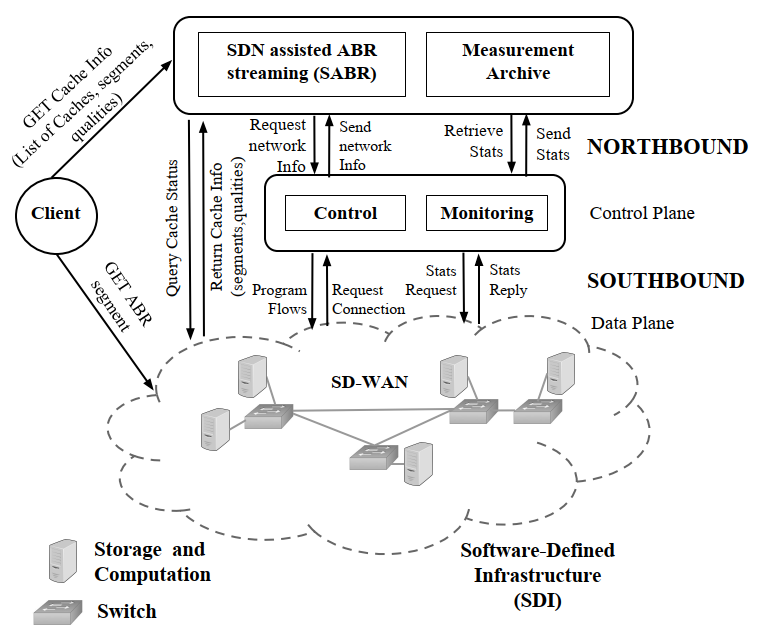
\includegraphics[scale=0.5]{images/sabr-arch.png}
\caption{SABR architecture design}
\label{fig:sabr}
\end{figure}

In general, the SABR architecture uses the information collected by the monitoring system to select the best cache in the network. This problem can be formalized as follows. Without loss of generality, we can consider an undirected weighted graph $G=(V, E)$ where $V$ is a set of network nodes, i.e., videos servers, switches, routers and stream clients. $E$ is the set of links between each networking node. Each edge $e \in E$ has a capacity $C(i,j)$ which represents the maximum network bandwidth. Given established routing, the available bandwidth between a client $i$ and a selected video cache server $j$ can be defined as

\begin{equation}
    R(i, j) = min_{(m,n) \in S(i,j)} C(m,n)
\end{equation}

where $S(i,j)$ is the set of all links belonging to the path between nodes $i$ and $j$. The physical meaning of this equation is that the download time of a given video segment for a given client is limited by the minimum bandwidth of intermediate nodes along the path. Thus, the adaptive quality adaptation problem for client $i$ can be formulated as

\begin{equation}
    T_{n,k} = min_{j \in G(n,k)} \frac{X_{n,k}}{R_{n,k}(i,j)}
\end{equation}

where $G(n,k)$ is the set of video cache servers that possess the segment $n$ with quality level $k$ which has the size $X_{n,k}$ in bits. Intuitively, the solution to this equation is to find the path with the highest available bandwidth between a given client and a set of video cache servers. 

However, bandwidth monitoring can only gives the observation of the past. By applying time-series analysis algorithms like Auto Regressive Integrated Moving Average (ARIMA), we can predict the future bandwidth bottleneck to help the clients determine the quality of the segments that should be retrieved next. In general, the SDN-assisted ABR streaming application utilizes this architecture to provide clients with accurate in-network available bandwidth information to archive video quality adaptation more efficiently.



% \newpage
\section{Our Implementation}
\subsection{Implementing SABR architecture on CloudLab}

The authors of \cite{bhat_network_2017} released their code of SABR implementation on GitHub \cite{sabr_code}. Our initial plan was to set up and run their code to reproduce the performance gain as claimed in the paper. However, during our experiments throughout previous weeks, we found their code is nigh unusable after five years. The reasons are listed as follows.

\subsubsection{OpenFlow monitoring}
As they've mentioned in Section 2.2 Monitoring Infrastructure \cite{bhat_network_2017}, accurate bandwidth monitoring of OpenFlow ports is one of the key components of the SABR design. In their implementation, they used SDN-OpenNetMon \cite{openmon}, an OpenFlow monitoring module based on the Pox controller developed by several researchers back in 2015. And since it's just an artifact of a research project, they never updated the SDN-OpenNetMon codebase since the paper's publication. Seven years later, the OpenFlow specification and Open vSwitch API has changed a lot, and SDN-OpenNetMon is not fully compatible with them anymore. 

So if we cannot get OpenFlow bandwidth monitoring working properly, we're missing the core component of this design. We had two options. The first option was debugging SDN-OpenNetMon, making it work properly with the current OpenFlow specification, Open vSwitch API, and Pox API. It's challenging since Pox is also not actively maintained anymore. The second option was that we develop an alternative to SDN-OpenNetMon on our own. Although it sounds complicated, it turns out to be relatively straightforward and much easier than debugging SDN-OpenNetMon. In our course project, we chose Ryu \cite{ryu} as the SDN framework since it's actively maintained, and widely used in production, and it provides detailed documentation and many examples. Ryu already provides an example of OpenFlow port monitoring (\url{https://github.com/faucetsdn/ryu/blob/master/ryu/app/simple_monitor_13.py}) so we just work on top of that. We followed the ideas of the original SABR code, after the bandwidth measurement is obtained, it's stored in a MongoDB database for future predictions. Although professional time-series database like InfluxDB might be more suitable for the task, we still use MongoDB in this project for the sake of simplicity. The code of our SDN controller can be found at \url{https://github.com/CSc579s22/Main/blob/master/server/controller.py}.

\subsubsection{Network topology}
In the original SABR implementation, many parameters and variables are hardcoded, including datapath IDs for OVS switches, client and server IPs, OpenFlow port numbers, network topologies, etc.  \url{https://github.com/dbhat/SABR/blob/master/controllerSABR/forwarding_cloudlab.py#L63-L133}. 

One reason why they hard coded such information might be that since they provided the CloudLab server topology (\url{https://github.com/dbhat/cloudlab_SABR/blob/master/profile.rspec}), theoretically, future researchers just have to provision servers using the same topology on CloudLab (because server IPs can also be defined in the CloudLab topology file), and they can reproduce the results without any problem. But it limits the scalability of their code, making it very difficult to apply their method on different server topologies. So we made our efforts to make it much more flexible. Our method is illustrated as follows.

Our Ryu controller maintains the network topology at any given time. Since every OVS bridge is connected to the Ryu controller using OpenFlow protocol, once a client is connected to an OVS bridge, the Ryu controller will automatically add it to the topology and start monitoring the corresponding port bandwidth. To do so, we used NetworkX \cite{networkx}, a Python package for the creation, manipulation, and study of the structure, dynamics, and functions of complex networks, to maintain the network topology as a weighted undirected graph $G=(V, E)$, where vertices $V$ includes streaming clients, cache servers and switches, edges $E$ are the corresponding connections between different nodes, and the edge weights are the measured bandwidth. NetworkX also provides useful functions such as shortest paths, which are used in the nearest cache server selection for clients. 

\subsubsection{Bandwidth prediction}
In the original SABR implementation, they used the \textit{auto.arima} function in the \textit{forecast} package provided by R programming language to predict future bandwidth for a given link, and they used \textit{rpy2} Python package as the bridge for calling R functions in Python. In our experiment, it's working fine if we just call R functions once, but if we call the same R functions multiple times within a loop, we will get the following error: \textit{Error in ts(x) : 'ts' object must have one or more observations}. Since we have no experience in R, after several failed attempts, we decided to use Python equivalent to replace R's \textit{auto.arima}. We found pmdarima \cite{pmdarima}, which claims provides the equivalent of R's \textit{auto.arima} functionality. 

\subsubsection{Caching and Caching Server Selection For Clients}
In the original SABR paper, they didn't mention many details about how to actually implement caching. They only mentioned in Section 5.2 Topology that they run a vanilla Apache2 web server along with an HTTP sniffer and a MongoDB database on cache nodes and together they implement an LRU cache replacement policy. The SABR code does not self-illustrate this issue in a clear way either. So we used Varnish \cite{varnish} instead, a reliable and fast caching HTTP reverse proxy. Varnish also uses LRU as the cache replacement policy. 

In Section 4.2 SDN Assisted Quality Adaptation \cite{bhat_network_2017}, they claimed that clients always choose the cache server with the highest available bandwidth. To do so, they measure $R_{n,k}(i,j)$, which denotes the available bandwidth during the download time of segment $X_{n,k}$. This measurement is based on the assumption that the network also carries other background traffic. 

In our implementation, we used our own approaches. For the initial cache server selection before downloading the first segment, the nearest cache server to the streaming client based on the minimum number of hops, i.e., the shortest path between the client and a list of available cache servers is returned to the client. This is archived by modifying the DASH player AStream, and sending requests to the Ryu controller to get the nearest cache server and the corresponding MPD file URL. After the playback starts, Ryu controller keeps monitoring bandwidth among all the paths and predicts future bandwidth using ARIMA. 

% The fairness metrics are calculated on each cache servers based on the current connected clients. 


\subsection{Implementing UFair on SABR}
We can implement the UFair model on SABR architecture in three internal stages:

\textbf{\underline{Stage 1}:} In the first stage, the continuous VQ utility functions is used to derive the optimal sharing of bandwidth which aims at an identical degree of video quality on all HAS streams. To achieve this goal, we need to solve the following equation:
\begin{equation}
\mathcal{U\prime}_{\text {res }}\left(r_{1}\right)=\mathcal{U\prime}_{\text {res }}\left(r_{2}\right)=\cdots=\mathcal{U\prime}_{\text {res }}\left(r_{N}\right) \quad \text { with } \quad r_{1}+r_{2}+\cdots+r_{2}=B W
\end{equation}

The output is a vector of bitrates, $\hat{R}=\left[\hat{r}_{1}, \hat{r}_{2}, \ldots, \hat{r}_{2}\right]$.

\textbf{\underline{Stage 2}:} In this stage by having $\hat{R}$ from the previous stage and MPD file, a bi-directional search of the nearest representation gets conducted. The MPD is a file that describes all of the resources and structure info required to stream a video. This file is given for implementation.

The search returns one or two playback rates for each $\hat{r}$ as $[[r_1^l,r_1^h ],...,[r_N^l,r_N^h ]]$. Each $[r_i^l,r_i^h]$ in the set represents the best approximation for optimal $\hat{r}_i$. The reason is, we don’t want the value of $\hat{r}_i$i be less than $r_i^l$ and more than $r_i^h$. 

Considering the output of this stage, now we can create a candidate list $C$, containing the $N$ streams in which each stream has one or two representations.

\textbf{\underline{Stage 3}:} Next, the candidate list gets evaluated with three fairness metrics. For each $c\in C$, we calculate each of the metrics $\mathfrak{J}^{V Q}$, $\mathfrak{J}^{S I}$ and $\mathfrak{J}^{C T}$, and then combine them to measure the user-level fairness. In order to aggregate fairness metrics in different scales, we rescale the fairness measurements using the maximum observed value as the rescaling factor. For instance, in the case of VQ metric:
\begin{equation}
\ddot{\mathfrak{J}}_{c}^{V Q}=\frac{\mathfrak{J}_{c}^{V Q}}{\max \left(\mathfrak{I}_{C}^{V Q}\right)}
\end{equation}

The value of this rescaled metric is between 0 and 1, where $\ddot{\mathfrak{J}}_{c}^{V Q}=1$ represents the worst solution from all candidates with respect to a given fairness measurement. 

We have applied this rescaling to all metrics and then combine them as following way:

$\ddot{\mathfrak{J}}_{c}^{\text {combined }}=\omega_{c}^{V Q} \times \ddot{\mathfrak{J}}_{c}^{V Q}+\omega_{c}^{S I} \times \ddot{\mathfrak{J}}_{c}^{S I}+\omega_{c}^{C T} \times \ddot{\mathfrak{J}}_{c}^{C T} ; \quad$ with $\omega_{c}^{V Q}+\omega_{c}^{S I}+\omega_{c}^{C T}=1$

The $\omega_c$ is the weight coefficient for each fairness metric and it defines how the fairness of video quality, switching impact and cost efficiency is balanced. This parameter is considered to be equal in the calculation for all metrics (which is equal to 1/3 for all metrics).
The candidate with minimum $\ddot{\mathfrak{J}}_{c}^{\text {combined }}$ is the best option to achieve the overall user-level fairness.

% All of these stages have been applied on the server side of SABR architecture. In such way that when the server receives the requests from clients, it starts the fairness calculation, and then sends the representation of the video as response so that maximize the fairness among clients. The implementation Python code of this section is available on our GitHub page (\url{https://github.com/CSc579s22/Main/blob/master/cache/fairness.py}).


% \newpage
\section{Performance evaluation}

We take reproducible research seriously. In the implementation of our course project, we tried to make our project easier to reproduce from many different aspects.

We implemented our experiments on CloudLab which is a research testbed platform \cite{Ricci2014IntroducingCS}. CloudLab supports the concept of \textit{Infrastructure as Code} that the network topology can be defined using Python library \textit{geni-lib}. Future researchers can recreate experiments with the same network topology using the same profile generated by Python scripts written in \textit{geni-lib}. The topology of our experiment is shown in Figure \ref{fig:ourarch} where the topology definition can be accessed at \url{https://github.com/CSc579s22/Main/blob/master/server/topology/fairness.py}.

\begin{figure}[H]
\centering
\includesvg[scale=0.5]{images/Arch.svg}
\caption{The Network Topology Used In Our Experiments}
\label{fig:ourarch}
\end{figure}

In our topology, we simulated a simplified version of multi-layer and multi-region CDN networks for adaptive video streaming. There is one origin video server that hosts the original copy of videos with different bitrate levels. We also install our SDN controller and MongoDB database on the origin video server. However, in practice, they can be installed on separate servers as well. For easier reproducibility, we packaged our SDN controller as a Docker image and provide a \textit{docker-compose.yaml} file which defines an application stack with SDN controller, MongoDB database for bandwidth measurement archive and Nginx for serving video requests. There are three software switches (sw1, sw2 and sw\_origin), which are implemented by installing Open vSwitch on vanilla Ubuntu virtual machines. There are two cache servers (cache1 and cache2) that serve the video requests for each group of streaming clients. Cache servers are implemented by installing Varnish HTTP Cache software \cite{varnish}. We also install the fairness metric calculation application on cache servers. There are six streaming clients, and each of them are connected to their regional switch.

The physical maximum bandwidth between virtual machines on CloudLab is 100MBps. In our experiment, we manually limit the maximum bandwidth to the values shown in Figure \ref{fig:ourarch}. The reason is as follows. We reused the test video dataset of \textit{BigBuckBunny} available at \url{http://ftp.itec.aau.at/datasets/DASHDataset2014/BigBuckBunny/2sec/}. The maximum available video bitrate is 4219897bps(approx. 4.2Mbps). The bandwidth limit on each link is implemented using Open vSwitch ingress policing and egress QoS. Based on our experiments, setting 500kbps limit on each client is suitable for the observation of network congestion and fairness competition. 

In our experiments, we compared three different ABR algorithms bundled with AStream under three different settings. The three ABR algorithms are \textit{Basic}, \textit{Netflix} and \textit{SARA} respectively. The \textit{Basic} algorithm is implemented by comparing the estimated download time of the next video segment with the current one. If the estimated download time of the next segment is longer then the client would request a lower bitrate. The \textit{Netflix} algorithm is an implementation of \cite{tyhuang}. The \textit{SARA} algorithm is the implementation of \cite{sara}. Note that AStream is released by the authors of \cite{sara} and they implemented \textit{Netflix} algorithm themselves. The three different settings are Baseline, SARA and Fairness. In Baseline, we let each client make ABR decisions solely and independently. In SABR, we redirect some clients to other idle cache servers. Specifically, \textit{sw1c3} and \textit{sw1c4} are connected to \textit{cache2} with a higher bandwidth of 10Mbps instead of their nearest cache server \textit{cache1}. In Fairness, we apply fairness calculation to enforce clients fetching the video segments with fair bitrates instead of their requested bitrates.

The performance evaluation is shown in Table \ref{tbl:baseline_sabr} and Table \ref{tbl:fairness} respectively. In Table \ref{tbl:baseline_sabr}, we compare the playback bitrate w.r.t playback time between Baseline and SABR. We can see that with less congestion, the average bitrates for all four clients are improved. However, the situation of rebuffering events and rebuffer time in Basic and SARA are not improved and may even become worse. Our interpretation is that the performance is still limited by the adaptive algorithm. 

In Table \ref{tbl:fairness}, we demonstrate the results when fairness is considered. In the first fairness setting, the four clients have the same maximum bandwidth of 500kbps. Thus the fairness calculation returns the same video bitrate for them. In the second fairness setting, the bandwidth limits from \textit{sw1c1} to \textit{sw1c4} are 200kbps, 400kbps, 600kbps and 800 kbps respectively. However, they still receive the same video bitrates. This is because we reused the MPD files provided by \cite{bhat_network_2017} and they only include 5 different video bitrates in total as shown in Table \ref{tbl:mpd_bitrate}. Since \cite{mu_scalable_2016} doesn't provide a utility function for 240p videos in Table \ref{video-utility}, we treat bitrate level 89283bps as 360p in our experiment as well, which might also affect the performance evaluation. The granularity of available video bitrates limits the fairness algorithm to select the most suitable video bitrate for each client, thus they receive the same video bitrate although the network capacity of each client is different. It's worth noting that in the setting of Fairness 2 in Table \ref{tbl:fairness}, since \textit{sw1c1} has the slowest network connection, it takes more time for it to stream the same video quality in the first 300 seconds. After 300 seconds, other clients have already finished playback, so the fairness calculation allocated 720p video with 791182bps for \textit{sw1c1}, which is way above its maximum bandwidth of 200kbps, thus causing many rebuffering events.
\\~\\

\begin{table}[H]
    \centering
    \begin{tabular}{|c|c|}
    \hline Resolution & Bitrate (bps) \\ \hline
       240p & 89283 \\ 
       360p & 262537 \\
       720p & 791182 \\
       1080p & 2484135, 4219897 \\
       \hline 
    \end{tabular}
    \caption{Available video bitrates defined in MPD files}
    \label{tbl:mpd_bitrate}
\end{table}

\begin{table}[H]
  \centering
  \begin{tabular}{ | m{1em} | c | c |}
    \hline
    & Baseline & SABR \\ \hline
    \parbox[t]{2mm}{\multirow{3}{*}{\rotatebox[origin=c]{90}{Basic}}}
    &
    \begin{minipage}{.45\textwidth}
      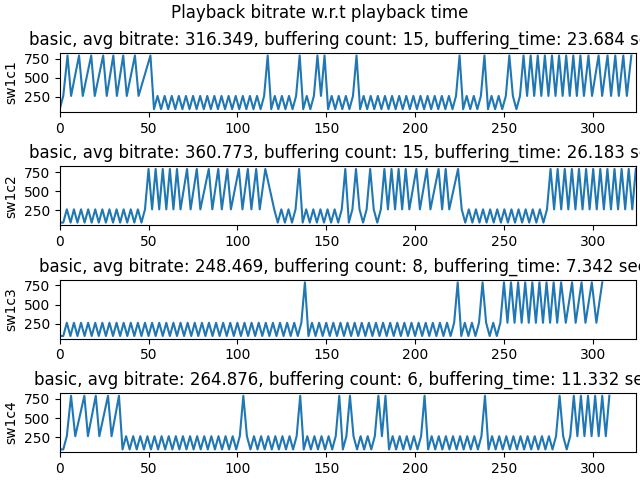
\includegraphics[width=\linewidth, height=60mm]{images/results/baseline_basic.png}
    \end{minipage}
    &
    \begin{minipage}{.45\textwidth}
      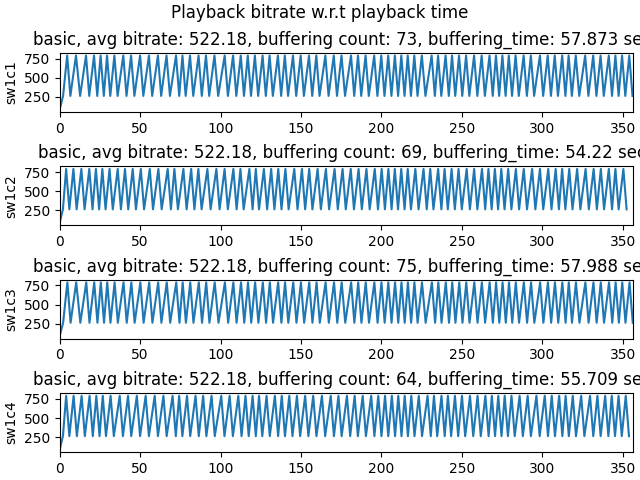
\includegraphics[width=\linewidth, height=60mm]{images/results/sabr_basic.png}
    \end{minipage}
    \\ \hline
    \parbox[t]{2mm}{\multirow{3}{*}{\rotatebox[origin=c]{90}{Netflix}}}
    &
    \begin{minipage}{.45\textwidth}
      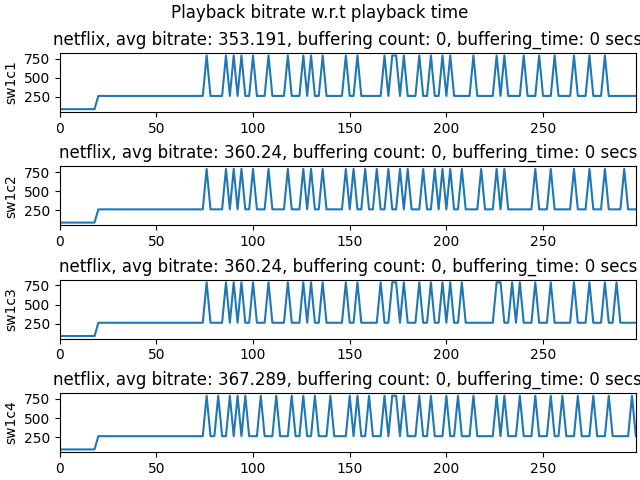
\includegraphics[width=\linewidth, height=60mm]{images/results/baseline_netflix.png}
    \end{minipage}
    & 
    \begin{minipage}{.45\textwidth}
      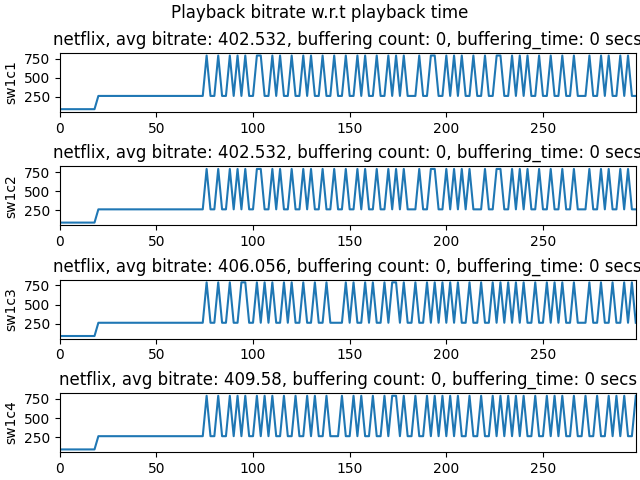
\includegraphics[width=\linewidth, height=60mm]{images/results/sabr_netflix.png}
    \end{minipage}
    \\ \hline
    \parbox[t]{2mm}{\multirow{3}{*}{\rotatebox[origin=c]{90}{SARA}}}
    &
    \begin{minipage}{.45\textwidth}
      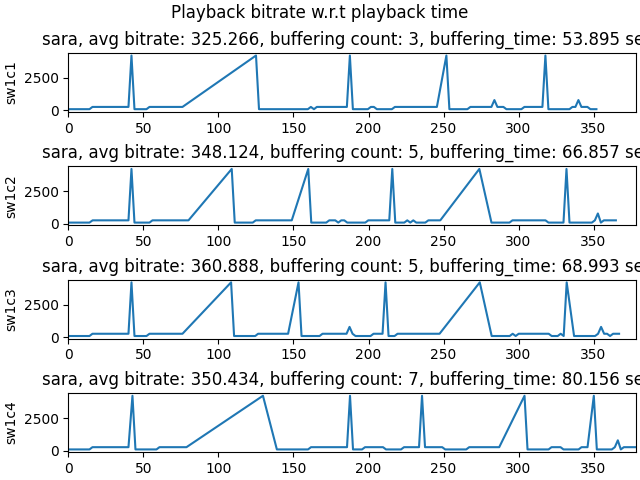
\includegraphics[width=\linewidth, height=60mm]{images/results/baseline_sara.png}
    \end{minipage}
    &
    \begin{minipage}{.45\textwidth}
      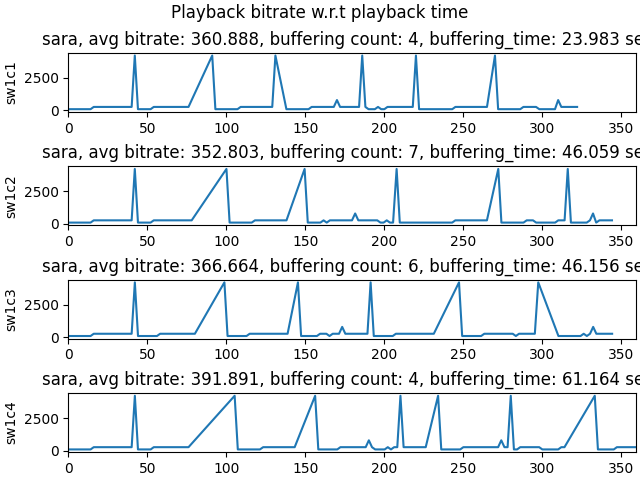
\includegraphics[width=\linewidth, height=60mm]{images/results/sabr_sara.png}
    \end{minipage}
    \\ \hline
  \end{tabular}
  \caption{Performance comparison between baseline and SABR. Each client has a maximum bandwidth of 500kbps.}\label{tbl:baseline_sabr}
\end{table}

\begin{table}[H]
  \centering
  \begin{tabular}{ | m{1em} | c | c |}
    \hline
    & Fairness 1  & Fairness 2 \\ \hline
    \parbox[t]{2mm}{\multirow{3}{*}{\rotatebox[origin=c]{90}{Basic}}}
    & 
    \begin{minipage}{.45\textwidth}
      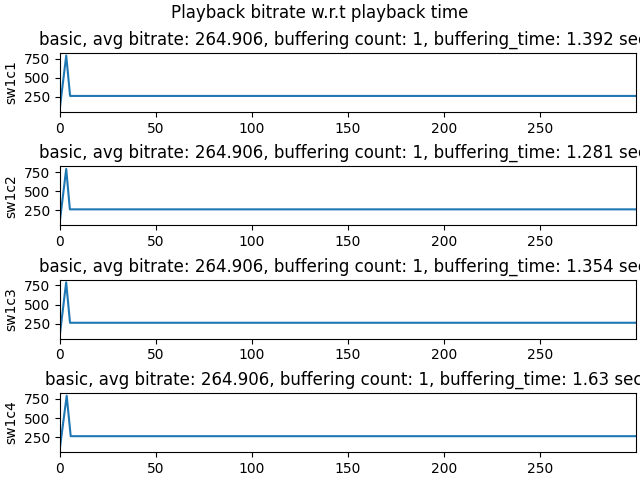
\includegraphics[width=\linewidth, height=60mm]{images/results/fairness_basic.png}
    \end{minipage}
    &
    \begin{minipage}{.45\textwidth}
      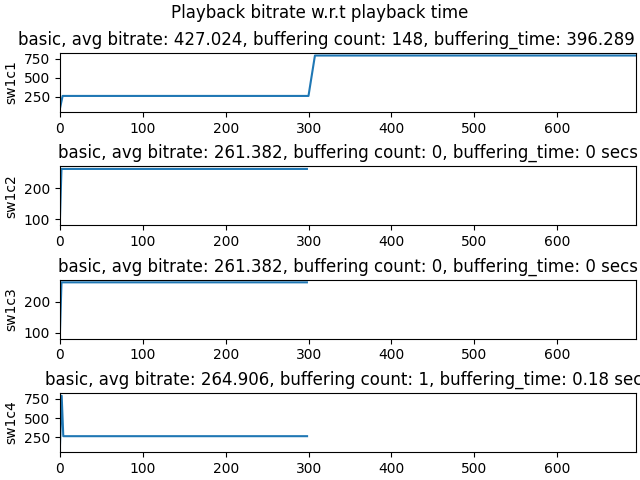
\includegraphics[width=\linewidth, height=60mm]{images/results/fairness_2_basic.png}
    \end{minipage}
    \\ \hline
    \parbox[t]{2mm}{\multirow{3}{*}{\rotatebox[origin=c]{90}{Netflix}}}
    &
    \begin{minipage}{.45\textwidth}
      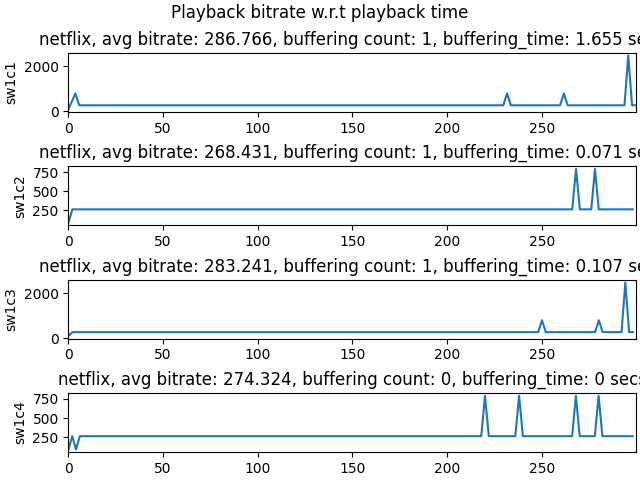
\includegraphics[width=\linewidth, height=60mm]{images/results/fairness_netflix.png}
    \end{minipage}
    & 
    \begin{minipage}{.45\textwidth}
      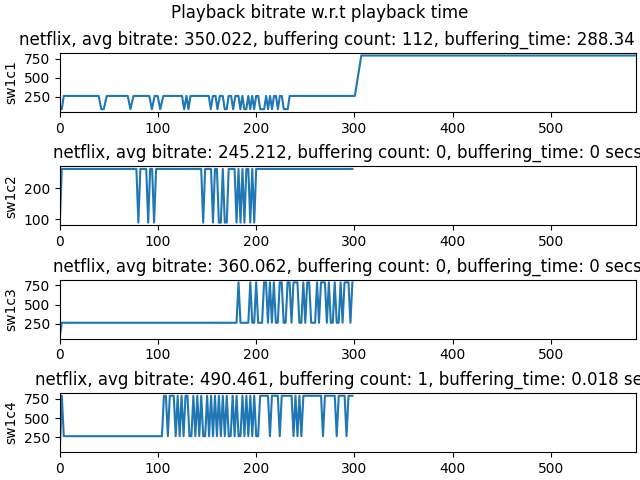
\includegraphics[width=\linewidth, height=60mm]{images/results/fairness_2_netflix.png}
    \end{minipage}
    \\ \hline
    \parbox[t]{2mm}{\multirow{3}{*}{\rotatebox[origin=c]{90}{SARA}}}
    &
    \begin{minipage}{.45\textwidth}
      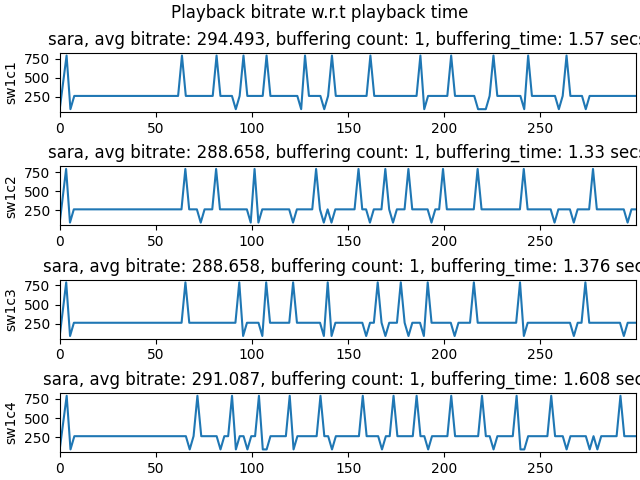
\includegraphics[width=\linewidth, height=60mm]{images/results/fairness_sara.png}
    \end{minipage}
    &
    \begin{minipage}{.45\textwidth}
      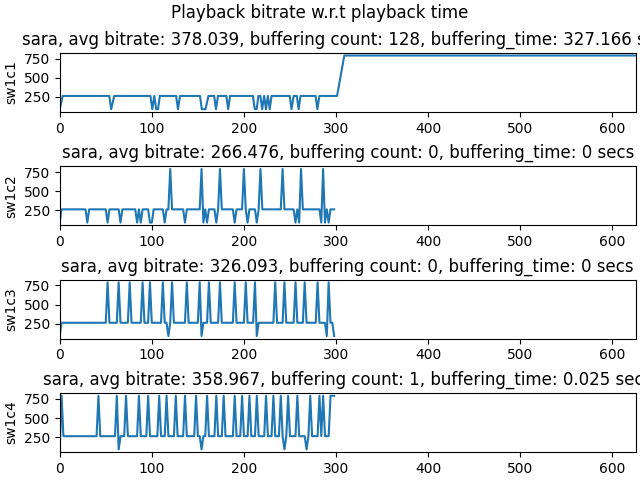
\includegraphics[width=\linewidth, height=60mm]{images/results/fairness_2_sara.png}
    \end{minipage}
    \\ \hline
  \end{tabular}
  \caption{Performance comparison between different fairness settings. In Fairness 1, each client has the same bandwidth limit of 500kbps. In Fairness 2, the bandwidth limits from sw1c1 to sw1c4 are 200kbps, 400kbps, 600kbps, and 800kbps respectively.}\label{tbl:fairness}
\end{table}

% \newpage
\section{Conclusion}
In this course project, we have investigated the software-defined infrastructure to provide an SDN control plane architecture that assists ABR video streaming applications in content delivery networks. In addition, we have tried to apply user-level fairness to SABR architecture so that maximizes the fairness between user experience on adaptive media streams. We have implemented our testbed on the CloudLab platform and applied the fairness at cache servers so that the cache server observes the fairness in responding to the client requests. Our results show that with the help of fair resource allocation, the QoE of the clients can be improved, although more comprehensive research needs to be done in future works, including but limited to set-up a more realistic scenario such as adding background network traffic, investigate the impact of different cache server placements and how to take the advantage of SDN and adaptive video streaming in real-world applications when an end-to-end SDN network is impossible with many intermediate networking devices.

% \newpage
\printbibliography[heading=bibnumbered]

\newpage

\addtocontents{toc}{\protect\setcounter{tocdepth}{1}}
\section{Appendix}

\subsection{Project Deliverables}
% \begin{table}
% \centering
\begin{center}
\begin{tabular}{ | m{20em} | m{18em} | } 
\hline
URL                                               & Note                                                                       \\ 
\hline
\url{https://github.com/CSc579s22/Main}                 & Main code repository                                                       \\ 
\hline
\url{https://github.com/CSc579s22/Visualization}        & Visualization scripts for performance evaluation                           \\ 
\hline
\url{https://github.com/CSc579s22/AStream}             & DASH player                                                                \\ 
\hline
\url{https://github.com/CSc579s22/UFair-Implementation} & Initial fairness metrics implementation which is later integrated into Main  \\ 
\hline
\url{https://github.com/CSc579s22/Documents}           & Archive of \LaTeX sources for documents                                                \\
\hline
\end{tabular}
\end{center}
% \end{table}

The DASH player AStream is forked from \url{https://github.com/pari685/AStream}. Other projects are implemented on our own.


\subsection{Member Contributions}
The Abstract, Section 1, Section 2 and Section 4.2 of this report are mainly contributed by Fatima Amri. 

Section 3, Section 4.1, Section 5 and Section 6 are mainly contributed by Jinwei Zhao. 

Fatima also has partial contributions to the draft of Section 3 and Section 6. 

Each member contributes evenly to the Project Proposal and every Bi-Weekly Update.

For contributions to the codes, Fatima contributed to the implementation of fairness metrics, the rest of the codes are implemented by Jinwei.

\end{document}
